\section{Motivação e Contexto Histórico}

Imagine a Europa do começo do século XVII, no período das grandes navegações, num mundo sem calculadoras nem computadores. Mas com a necessidade de se computar operações (especialmente multiplicações e divisões) com números grandes, e cada vez maiores, surgiu a necessidade de se fazer isso cada vez mais rápido.

A primeira ideia, ao invés de tentar criar uma máquina que fizesse as contas, foi tentar simplificar o problema. No século XVI, nasce a ideia de "transformar o produto em uma soma", utilizando a \textit{trigonometria}. Mais precisamente, era utilizada as relações de Prostraférese, como a que segue:

\[
    2\cos(a)\cos(b) = \cos(a + b) + cos(a - b)
\]

Com essa ideia, e uma tabela trigonométrica, multiplicações de números poderiam ser feitas rapidamente, trocando-as por somas, e consultas à tabela, podemos fazer um exemplo breve:

Imagine que queremos realizar o seguinte produto: $0,98374 \cdot 0,90923$, utilizando de uma tabela trigonométrica, podemos fazer:
\[
\begin{gathered}
\begin{cases} 2 \cos a = 0,98374 \\ \cos b = 0,90923 \end{cases} \Rightarrow \begin{cases} a \cong 60^\circ \\ b \cong 25^\circ \end{cases} \Rightarrow \cos(a + b) + \cos(a - b) = \\ \cos(85^\circ) + \cos(35^\circ) = 0,0872 + 0,8192 = 0,9064
\end{gathered}
\]

Multiplicando com uma calculadora dos tempos atuais obtemos: $0,8944459202$. O Resultado encontrado era muito preciso para a época, e que não custou um esforço muito grande a não ser somar e substituir valores de uma tabela. Esse método foi muito utilizado por matemáticos e astrônomos da época.

Essas ideias de transformar multiplicação para soma, abriu porta para um novo conceito: \textit{Os logaritmos}

\subsection{John Napier}

\begin{wrapfigure}{l}{0.3\textwidth}
    \setlength{\intextsep}{0pt}
    \vspace{-1.5em} 
    \centering
    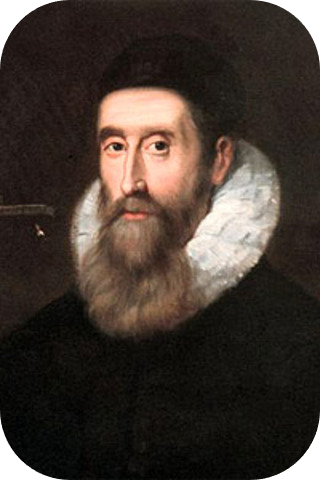
\includegraphics[width=\linewidth]{img/napier.png} 
\end{wrapfigure}

John Napier (1550-1617) foi um proprietário escocês, nascido no castelo de Merchinston, na Escócia. John Napier teve origem nobre, viveu a maior parte de sua vida na majestosa propriedade de sua família. Era constantemente envolvido com controvérsias políticas e religiosas, e era anticatólico declarado. Em 1593 tentou provar numa publicação que o Papa era o Anticristo. Esta publicação atingiu 21 edições, com pelo menos dez ainda em vida do autor.

% Conta-se várias histórias sobre Napier, uma delas conta que seu galo negro teria identificado para ele os empregados que o roubavam. Um a um os empregados foram enviados a um quarto escuro com instruções para tocar no dorso do galo. Porém, sem que os empregados soubessem, Napier cobriu o dorso da ave com uma fuligem, e os empregados culpados, tremendo tocar no galo, voltavam com as mãos limpas.


Napier desenvolveu um método similar ao da Prostraférese, na verdade, acredita-se que Napier tenha se influenciado por ele para criar seu método, pois ele utilizava tabelas de senos e seus ângulos. Apesar de não existir a notação exponencial, Napier fez a seguinte abordagem: Associou os termos das progressões geométricas e aritméticas da tabela abaixo:


\begin{table}[h]
\centering
\renewcommand{\arraystretch}{1.2} 
\begin{tabular}{|c|c|c|c|c|c|c|c|c|}
\hline
$b^1$ & $b^2$ & $b^3$ & $b^4$ & $\dots$ & $b^m$ & $\dots$ & $b^n$ & $\dots$ \\
\hline
1 & 2 & 3 & 4 & $\dots$ & $m$ & $\dots$ & $n$ & $\dots$ \\
\hline
\end{tabular}
\end{table}

\noindent 
então o produto de dois termos $b^m b^n$ da primeira progressão está associado à soma $m + n$ dos termos da segunda progressão.

Por exemplo, imagine que temos uma tabela com todas as potências de 2 e queremos realizar o produto: $512 \cdot 1024$, observe que isto é igual a $2^9 \cdot 2^{10}$, esse termo da progressão geométrica está associado ao termo $10 + 9 = 19$ da progressão aritmética, portanto, basta olhar na tabela quem é o número $2^{19}$, e assim, conseguimos calcular o produto sem precisar efetuar nenhuma multiplicação.

Napier utilizou dessa ideia. Para manter os termos da progressão geométrica suficiente próximos, adotou $b = 1 - \frac{1}{10^7} \approx 1$, então seu decrescimento é lento o suficiente para termos bem próximos. Além disso, para evitar decimais, Napier multiplicou cada termo por $10^7$. Então, a tabela agora poderia ser reescrita da seguinte forma:

\begin{table}[h]
\centering
\renewcommand{\arraystretch}{1.2} 
\begin{tabular}{|c|c|c|c|c|c|c|c|c|}
\hline
$9999999$ & $9999998$ & $9999997$ & $\dots$ & $9999900$ & $\dots$ & $3678794,228$ & $\dots$ \\
\hline
1 & 2 & 3 & $\dots$ & $100$ & $\dots$ & $10000000$ & $\dots$ \\
\hline
\end{tabular}
\end{table}


Daí, para qualquer $N$ da primeira progressão, existe um único $L$ na segunda progressão, de modo que
$$
N = 10^7 \left(1 - \frac{1}{10^7}\right)^L
$$
Napier chamava $L$ de logaritmo de $N$, e definiremos $\operatorname{Naplog} N = L$.

Napier publicou sua abordagem dos logaritmos em 1614 num texto intitulado \textit{Mirifici Logarithmorum Canonis Descriptio} (Descrição da Maravilhosa Lei dos Logaritmos). O trabalho contém uma tábua que dá os logaritmos dos senos de ângulos para minutos sucessivos de arco.

\begin{figure}[H]
    \centering
    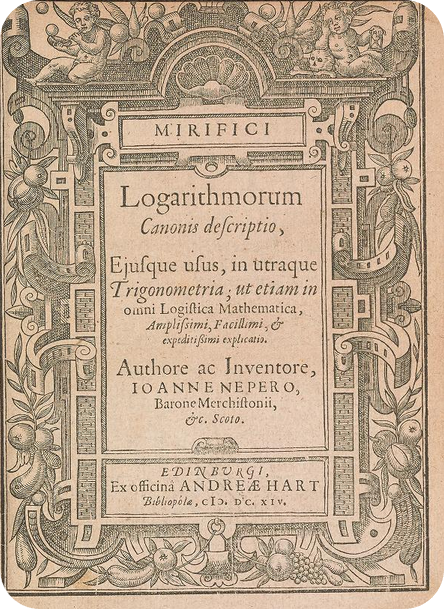
\includegraphics[height=9cm]{img/mirificiLog.png}
    \caption{Capa do Mirifici Logarithmorum Canonis Descriptio}
\end{figure}

\begin{figure}[H]
    \centering
    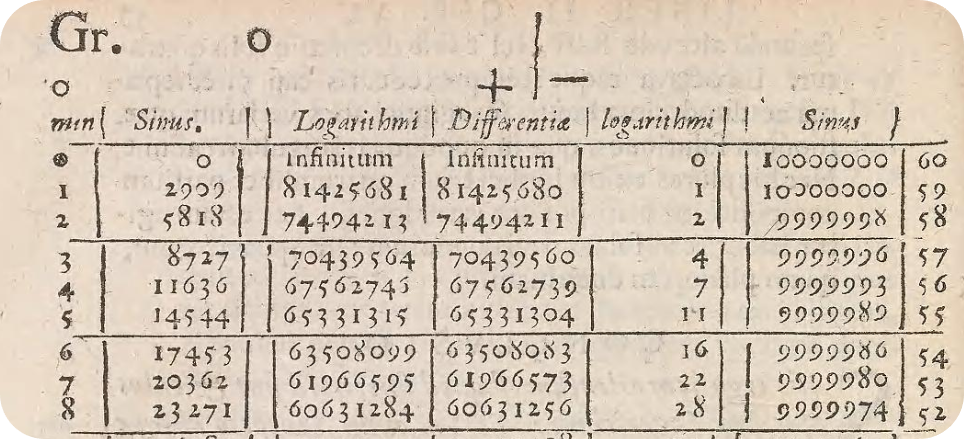
\includegraphics[height=4.5cm]{img/tabelanapier.png}
    \caption{Tabela desenvolvida por Napier}
\end{figure}